%% Author: Leighton Pritchard
%% Copyright: James Hutton Institute
%% This presentation was an invited guest lecture on microbial genomics and bioinformatics
%% for the BM405 course.

%% GENERIC STYLE SETTINGS BELOW
\usetheme{default}
\usepackage{listings}
\usepackage{multirow}
\usepackage{xcolor}
\usepackage{hyperref}

\usebackgroundtemplate{

\includegraphics[width=\paperwidth,height=\paperheight]{images/hutton_background}
}
%% PRESENTATION CONFIGURATION PARAMETERS %%%%%%%%%%%%%%%%%%%%%%%%%%%%%%%%%%%%%%%
%\titlebackgroundfile{images/hutton_title}
%\framebackgroundfile{images/hutton_background}
\definecolor{hutton_green}{HTML}{78A22F}
\definecolor{hutton_purple}{HTML}{872175}
\definecolor{hutton_blue}{HTML}{569BBE}
\usefonttheme{structurebold}
\setbeamercolor{alerted text}{fg=orange}
\setbeamercolor{background canvas}{bg=white}
\setbeamercolor{block title}{bg=hutton_purple}
\setbeamercolor{frametitle}{fg=hutton_purple}
\setbeamercolor{title}{fg=black}
\setbeamercolor{titlelike}{fg=hutton_green}
\setbeamercolor{author}{fg=hutton_purple}
\setbeamercolor{author in head/foot}{fg=white}
\setbeamercolor{title in head/foot}{fg=white}
\setbeamercolor{section in head/foot}{fg=hutton_purple}
\setbeamercolor{normal text}{fg=black}
\setbeamercolor{frametitle}{fg=hutton_purple}
\setbeamerfont{block title}{size={}}
\setbeamerfont{author}{size=\footnotesize}
\setbeamerfont{institute}{size=\tiny}
\setbeamerfont{date}{size=\footnotesize}
\setbeamercolor{section in toc shaded}{fg=hutton_purple}
\setbeamercolor{section in toc}{fg=hutton_purple}
\setbeamercolor{subsection in toc shaded}{fg=hutton_purple}
\setbeamercolor{subsection in toc}{fg=hutton_purple}
\setbeamertemplate{itemize item}[circle]
\setbeamertemplate{itemize subitem}[circle]
\setbeamertemplate{itemize subsubitem}[circle]
\setbeamertemplate{itemize subsubsubitem}[circle]
\setbeamercolor{itemize item}{fg=hutton_purple}
\setbeamercolor{itemize subitem}{fg=hutton_purple}
\setbeamercolor{itemize subsubitem}{fg=hutton_purple}
\setbeamercolor{itemize subsubsubitem}{fg=hutton_purple}
\setbeamercolor{enumerate item}{fg=hutton_purple}
\setbeamercolor{enumerate subitem}{fg=hutton_purple}
\setbeamercolor{enumerate subsubitem}{fg=hutton_purple}
\setbeamercolor{enumerate subsubsubitem}{fg=hutton_purple}
\setbeamercolor{alerted text}{fg=hutton_green}
\setbeamerfont{alerted text}{series=\bfseries}
% This command makes sure that acrobat reader doesn't change the colours of the slide
% when there are figures with transparencies.
\pdfpageattr {/Group << /S /Transparency /I true /CS /DeviceRGB>>}

%Disables discrete bottom navigation bar
%\beamertemplatenavigationsymbolsempty

% Modify the slide titles to avoid the corner images,
\setbeamertemplate{frametitle}
{
\vspace{0.05\textheight}
\noindent\quad\begin{minipage}[t][0.12\textheight][t]{0.85\textwidth}
\insertframetitle\par
\end{minipage}
}

% Modify title page to avoid the big logo on right
\setbeamertemplate{title page}{
    \begin{picture}(0,0)
            %This ends up on top of the default background image, rather than replacing it:
            \put(-30,-165){%
                
\includegraphics[width=\paperwidth,height=\paperheight]{images/hutton_title}
            }
            \put(0,-75){%
                \begin{minipage}[b][0.4\textheight][t]{0.75\textwidth}
                    \usebeamerfont{title}\usebeamercolor[fg]{title}{\inserttitle\par}
                    \usebeamerfont{subtitle}\usebeamercolor[fg]{subtitle}{\insertsubtitle\par}
                \end{minipage}
            }
            \put(0,-125){%
                \begin{minipage}[b][0.1\textheight][t]{\textwidth}
                    \usebeamerfont{author}\usebeamercolor[fg]{author}{\insertauthor\par}
                    \usebeamerfont{institute}\usebeamercolor[fg]{institute}{\insertinstitute\par}
                \end{minipage}
            }
    \end{picture}
}

%%%%%%%%%%%%%%%%%%%%%%%%%%%%%%%%%%%%%%%%%%%%%%%%%%%%%%%%%%%%%%%%%%%%%%%%%%%%%%%%

% LISTINGS SETTING
% Settings for code listings in lstlistings

\definecolor{hutton_lightgreen}{HTML}{C8F27F}

\lstset{ %
  backgroundcolor=\color{hutton_lightgreen},   % choose the background color; you must add \usepackage{color} or \usepackage{xcolor}
  basicstyle=\tiny\ttfamily,        % the size of the fonts that are used for the code
  breakatwhitespace=false,         % sets if automatic breaks should only happen at whitespace
  breaklines=true,                 % sets automatic line breaking
  captionpos=b,                    % sets the caption-position to bottom
  commentstyle=\color{red},    % comment style
  deletekeywords={...},            % if you want to delete keywords from the given language
  escapeinside={\%*}{*)},          % if you want to add LaTeX within your code
  extendedchars=true,              % lets you use non-ASCII characters; for 8-bits encodings only, does not work with UTF-8
  frame=single,                    % adds a frame around the code
  keepspaces=true,                 % keeps spaces in text, useful for keeping indentation of code (possibly needs columns=flexible)
  keywordstyle=\color{blue},       % keyword style
%  language=Octave,                 % the language of the code
  morekeywords={*,...},            % if you want to add more keywords to the set
  numbers=left,                    % where to put the line-numbers; possible values are (none, left, right)
  numbersep=5pt,                   % how far the line-numbers are from the code
  numberstyle=\tiny\color{gray}, % the style that is used for the line-numbers
  rulecolor=\color{black},         % if not set, the frame-color may be changed on line-breaks within not-black text (e.g. comments (green here))
  showspaces=false,                % show spaces everywhere adding particular underscores; it overrides 'showstringspaces'
  showstringspaces=false,          % underline spaces within strings only
  showtabs=false,                  % show tabs within strings adding particular underscores
  stepnumber=1,                    % the step between two line-numbers. If it's 1, each line will be numbered
  stringstyle=\color{violet},     % string literal style
  tabsize=4,                       % sets default tabsize to 2 spaces
  title=\lstname                   % show the filename of files included with \lstinputlisting; also try caption instead of title
}


%%%
% TITLE PREAMBLE
\title[Microbial Genomics and Bioinformatics: 3.Whole Genome Comparisons] % (optional, only for long titles)
{Microbial Genomics and \\ Bioinformatics \\
BM405 \\
3.Whole Genome Comparisons}
%\subtitle{}
\author[Pritchard] % (optional, for multiple authors)
{Leighton~Pritchard$^{1,2,3}$}
\institute[The James Hutton Institute] % (optional)
{
  $^{1}$Information and Computational Sciences,\\
  $^{2}$Centre for Human and Animal Pathogens in the Environment,\\
  $^{3}$Dundee Effector Consortium,\\
  The James Hutton Institute, Invergowrie, Dundee, Scotland, DD2 5DA
}
\subject{Bioinformatics, Genomics, Bacteria, Sequencing, Microbiology, Microbes}

%%%
% TOC
% Show table of contents, with current section highlighted,
% at the start of each section

%\AtBeginSection[]
%{
%  \begin{frame}
%    \frametitle{Table of Contents}
%    \tableofcontents[currentsection] %,hideallsubsections]
%  \end{frame}
%}

\AtBeginSubsection[]
{
  \begin{frame}
    \frametitle{Table of Contents}
    \tableofcontents[currentsection,currentsubsection] %,hideallsubsections]
  \end{frame}
}

%%%
% START DOCUMENT
\begin{document}

\frame[plain]{\titlepage}

%% use.tex
%% Author: Leighton Pritchard
%% Copyright: James Hutton Institute
%% These slides describe the acceptable use policy for these slides and
%% materials

%
\begin{frame}
  \frametitle{Acceptable Use Policy}
  Recording of this talk, taking photos, discussing the content using \\
  email, Twitter, blogs, etc. is permitted (and encouraged), \\
  providing distraction to others is minimised. \\[0.5cm]
  These slides will be made available on SlideShare. \\[0.5cm]
  These slides, and supporting material, are available at \href{https://github.com/widdowquinn/Teaching-2014-11-21-Strathclyde}{https://github.com/widdowquinn/Teaching-2014-11-21-Strathclyde}
\end{frame}

%%%
% SECTION: Comparative Genomics
\section{Comparative Genomics}
%% comparative_genomics_intro.tex
%% Author: Leighton Pritchard
%% Copyright: James Hutton Institute
%% A brief description of the power of comparative genomics

% SUBSECTION: What you get back
% What you get back from assembly
\subsection{Computational Comparative Genomics}

% What computational comparative genomics gives you
\begin{frame}
  \frametitle{The Power of Comparative Genomics}
  Massively enabled by high-throughput sequencing, and the availability of thousands of sequenced isolates.\\[0.5cm]
  Computational comparisons more powerful and precise than experimental comparative genomics: \textbf{the ultimate microbial typing solution}\\[0.5cm]
  Three broad areas/scales:
  \begin{itemize}
    \item Comparison of bulk genome properties
    \item Whole genome sequence comparisons
    \item \textit{Comparison of features/functional components}
  \end{itemize}    
\end{frame}

% Bulk genome properties
\begin{frame}
  \frametitle{Bulk Genome Properties}
  Not taking sequence order/structure into account
  \begin{columns}[T]
    \begin{column}{5cm}
      \begin{itemize}
        \item Chromosome and plasmid counts
        \item Chromosome and plasmid sizes
        \item Nucleotide content
        \item $k$-mer content
      \end{itemize}    
      Classification/discrimination of sequences\\
    \end{column}
    \begin{column}{5cm}
      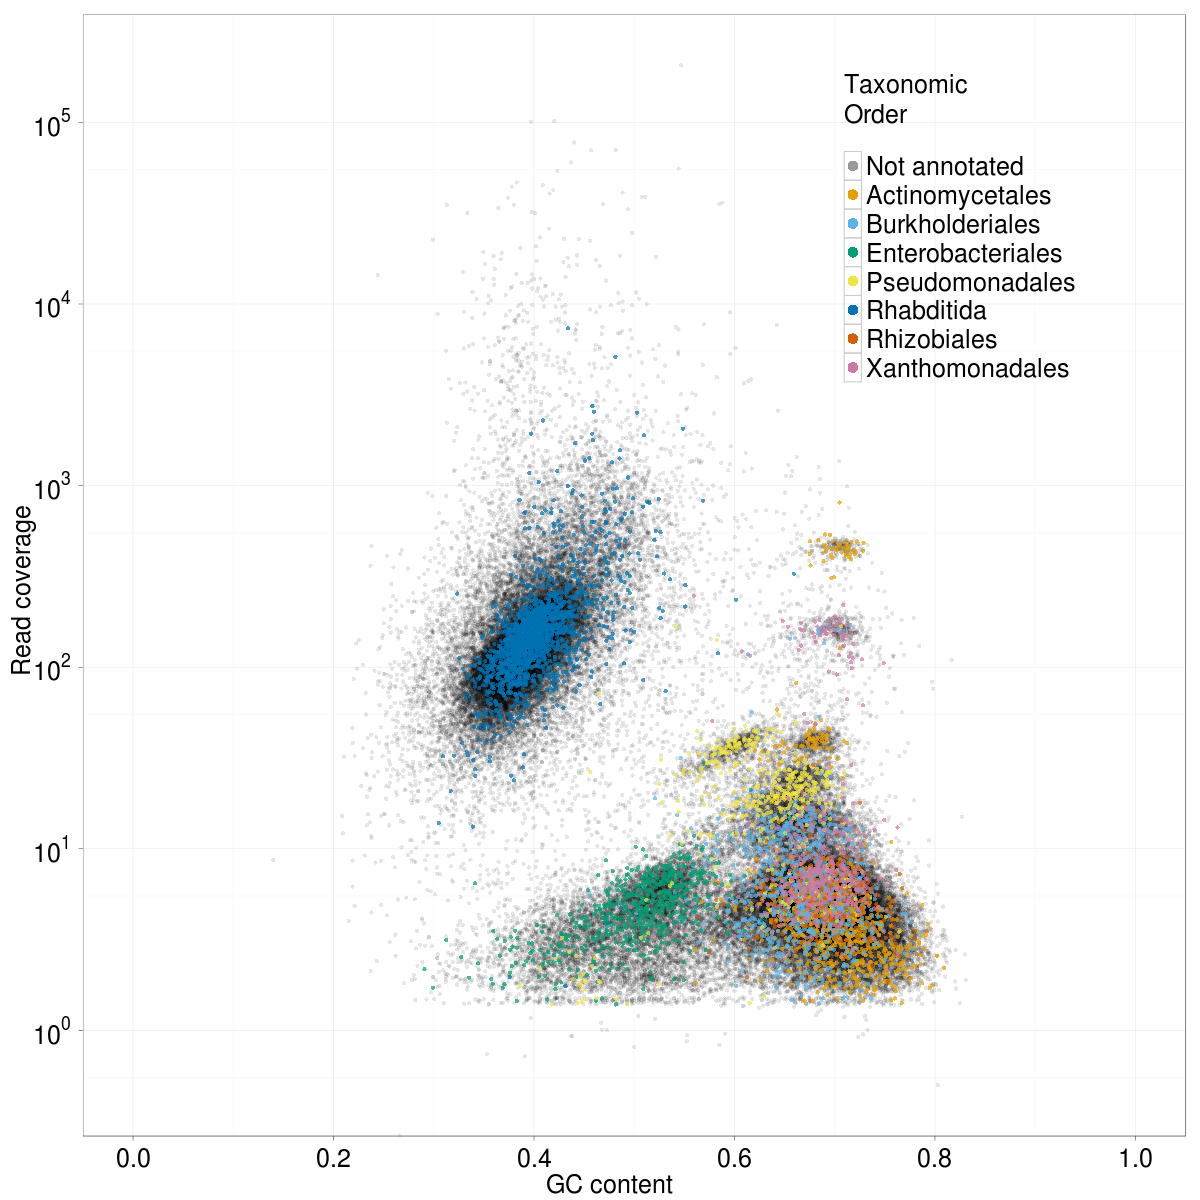
\includegraphics[width=1\textwidth]{images/blobology}
    \end{column}
  \end{columns}
\end{frame}

% Whole genome sequence comparisons
\begin{frame}
  \frametitle{Whole Genome Sequences}
  Introduces sequence order and structure
  \begin{itemize}
    \item Whole genome similarity
    \item Identification of sequence-similar regions
    \item Rearrangements
    \item Insertions/deletions
  \end{itemize}    
  Genome structure/evolution, and taxonomic classification.
  \begin{center}
    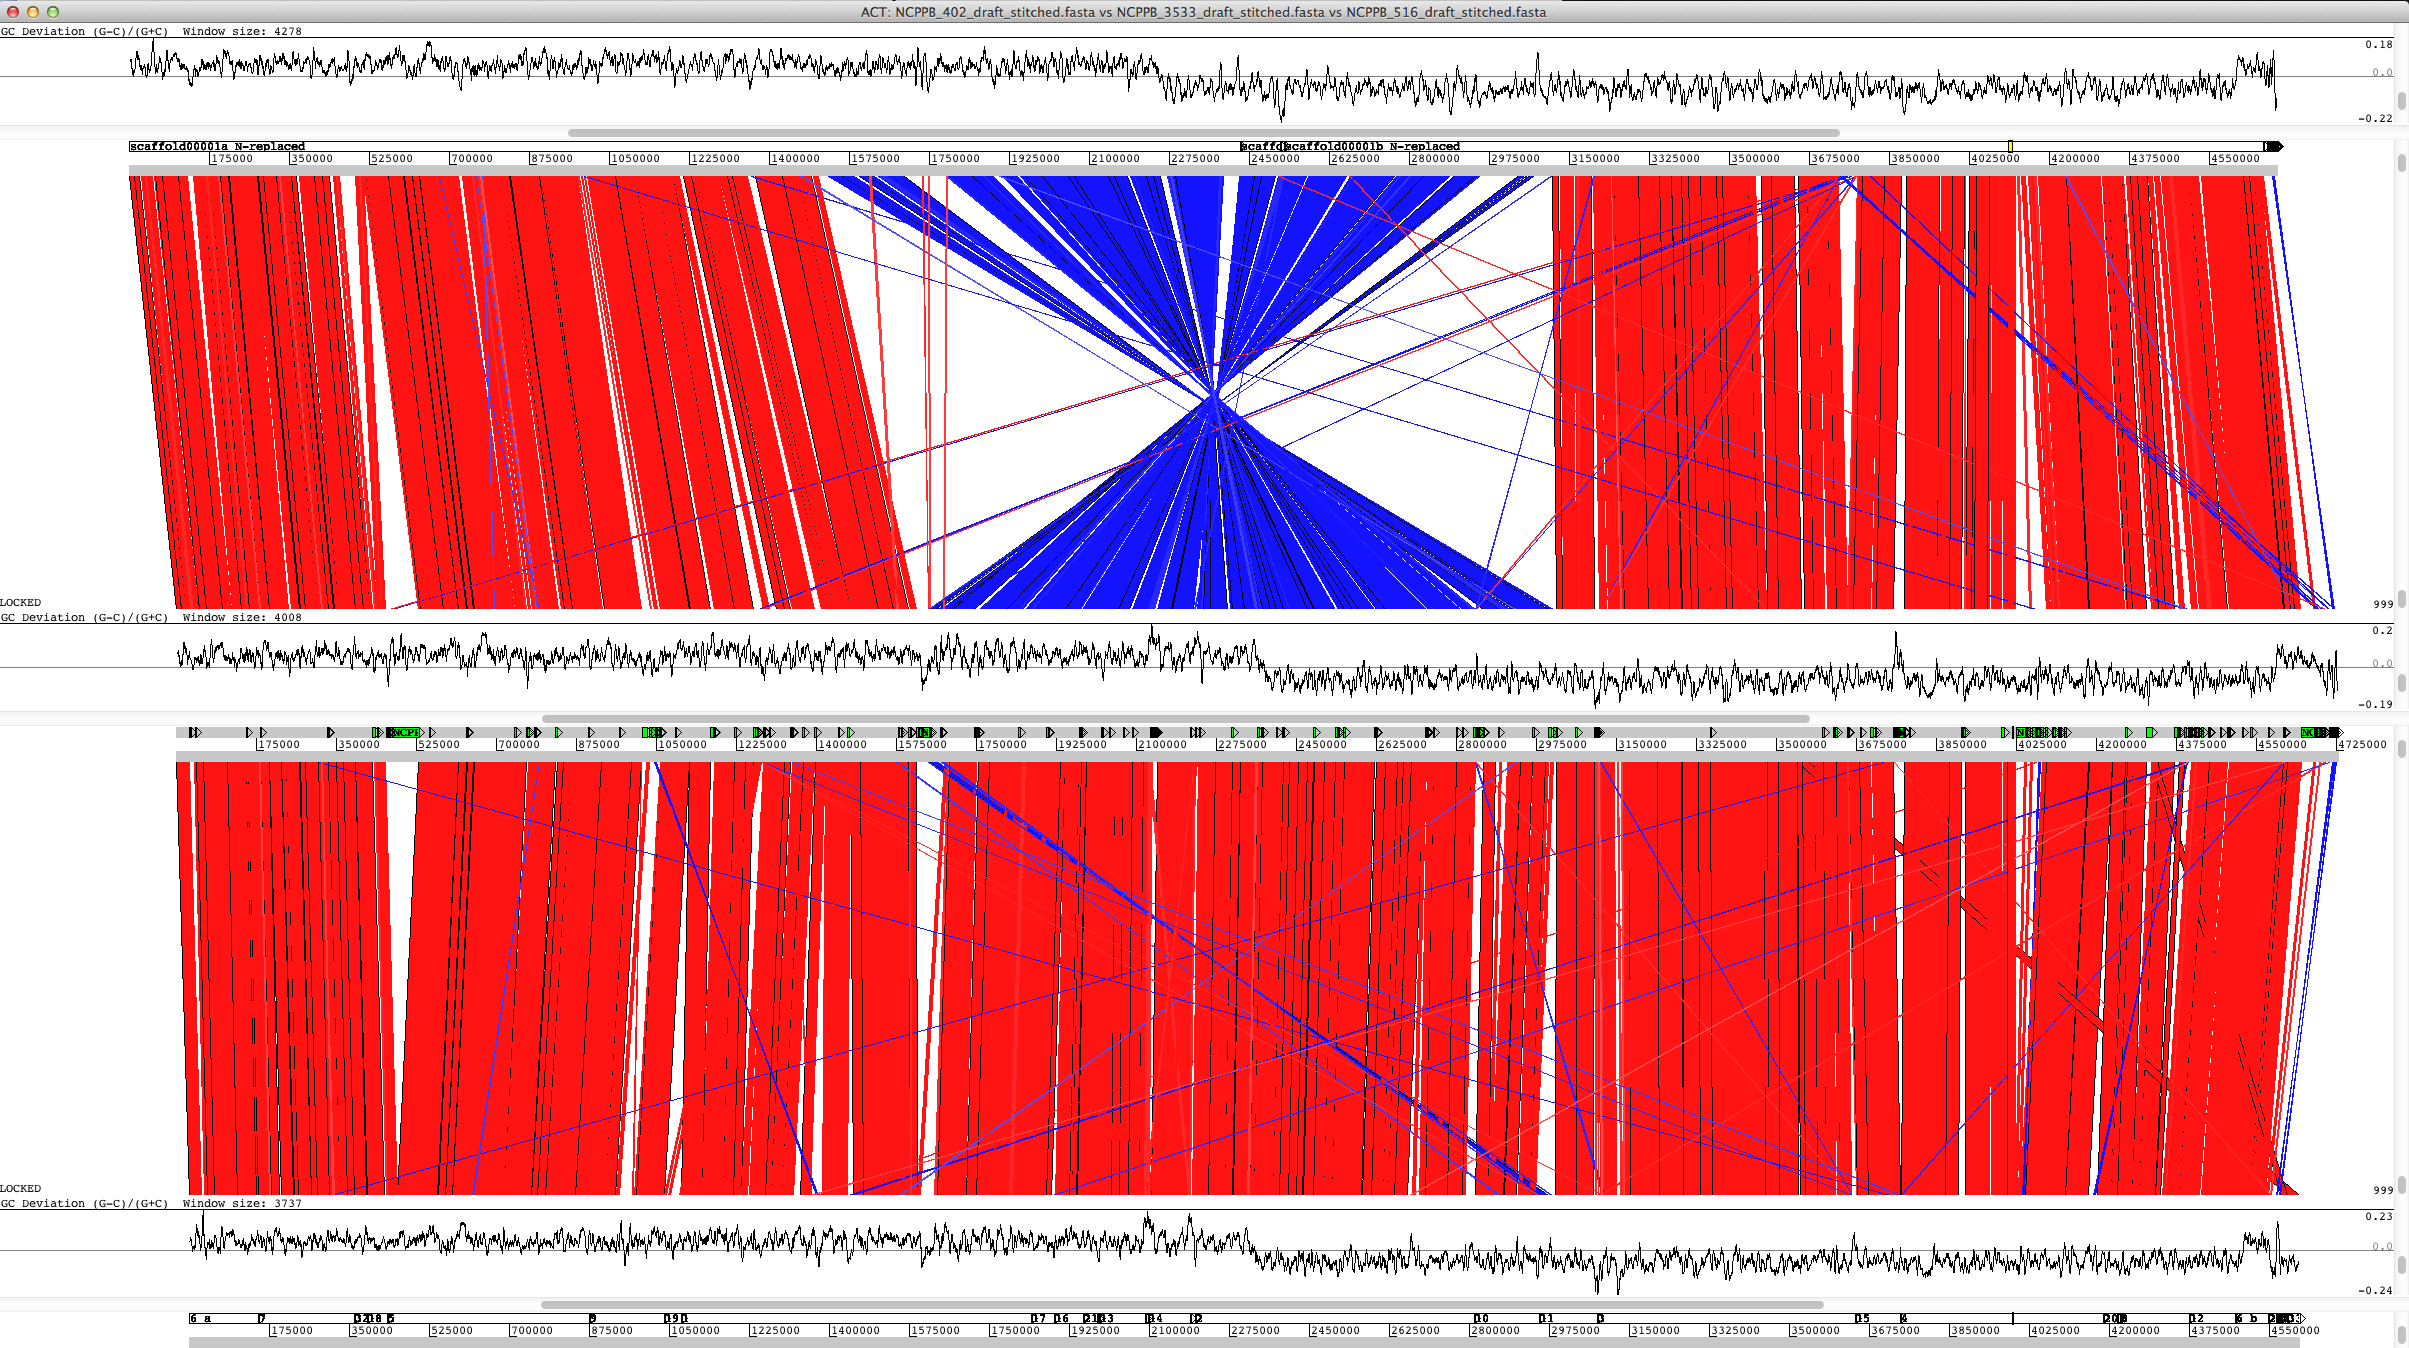
\includegraphics[height=0.4\textheight]{images/act_comparison}
  \end{center}  
\end{frame}

% Genome features and functional components
\begin{frame}
  \frametitle{Genome Feature Comparisons}
  Introduces functional elements, sequence subregions
  \begin{columns}
    \begin{column}{5.5cm}
      \begin{itemize}
        \item Numbers and types of features (genes, ncRNA, regulatory elements, etc.)
        \item Organisation of features (synteny, operons, etc.)
        \item Inference of functional/phenotypic differences
        \item Inference of selection pressure and adaptation
      \end{itemize}  
      Functional capacity, modifications/adaptations of biochemistry and phenotype  
    \end{column}
    \begin{column}{5cm}
      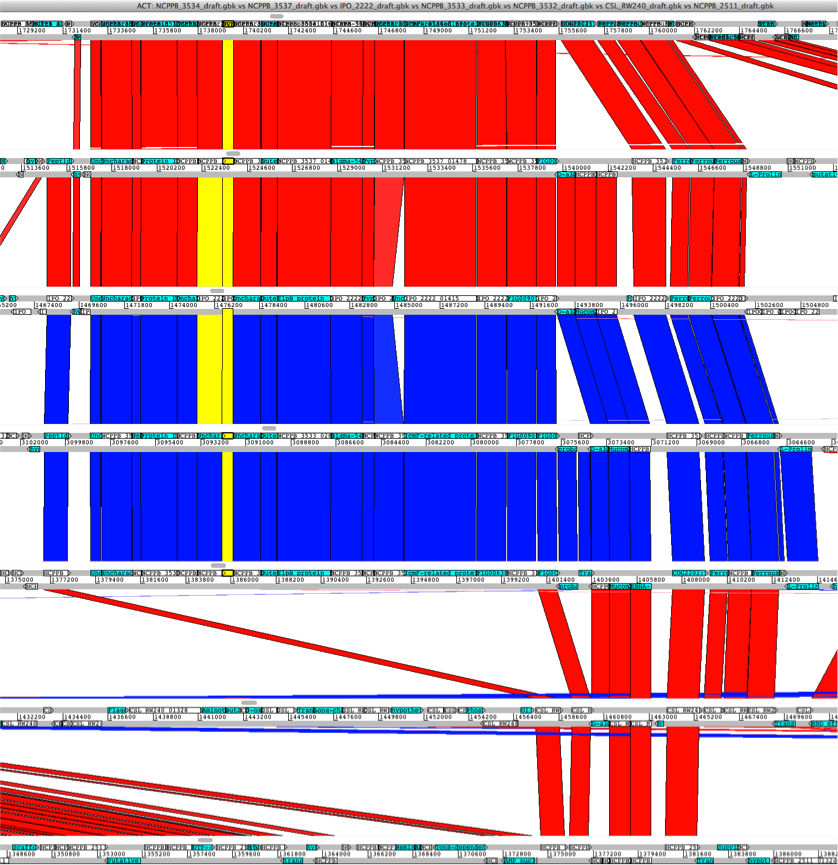
\includegraphics[width=1\textwidth]{images/t6ss}    
    \end{column}
  \end{columns}
\end{frame}

%%%
% SECTION: Bulk Genome Properties
\section{Bulk Genome Properties}
%% bulk_genome_properties.tex
%% Author: Leighton Pritchard
%% Copyright: James Hutton Institute
%% A brief description of useful bulk genome properties

% SUBSECTION: Nucleotide frequency and genome size
\subsection{Nucleotide Frequency/Genome Size}

% Calculating GC content/skew
\begin{frame}
  \frametitle{Nucleotide frequency/genome size}
  \begin{itemize}
    \item Very easy to calculate from complete/draft genome
    \item Can calculate for individual contigs/scaffolds/regions
    \item Usually reported in GUI genome browsers
  \end{itemize}    
  Trivial to determine using, e.g. Python
  \begin{center}
    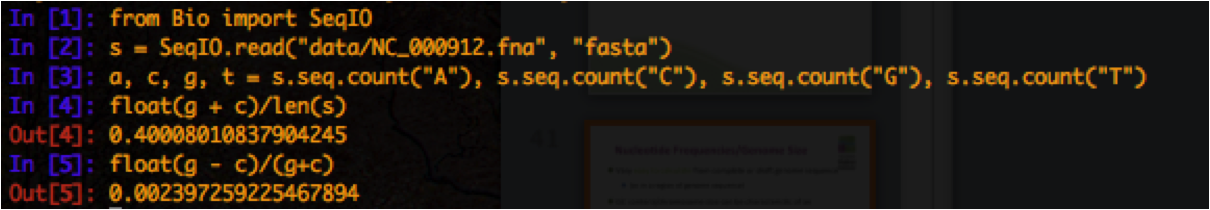
\includegraphics[width=1\textwidth]{images/python_gc}
  \end{center}  
\end{frame}

% GC content and genome size
\begin{frame}
  \frametitle{Nucleotide frequency/genome size}
  GC content and chromosome size can be characteristic\\
  See \texttt{data/bacteria\_size} for example iPython notebook exercise\\[0.5cm]
  \begin{center}
    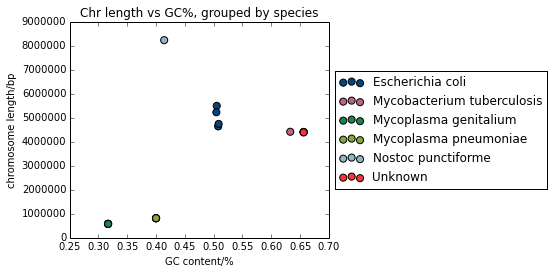
\includegraphics[width=1\textwidth]{images/gc_vs_size}
  \end{center}  
\end{frame}

% Blobology
\begin{frame}
  \frametitle{Blobology\footnote{\tiny{\href{http://dx.doi.org/10.1007/s13199-012-0154-6}{Kumar and Blaxter \textit{et al}. (2011) \textit{Symbiosis} \textbf{3}:119-126 doi:10.1007/s13199-012-0154-6}}}}
  \begin{columns}[T]
    \begin{column}{5cm}
      Sequencing samples may be contaminated or contain microbial symbionts.\\
      Expect more host than symbiont/contaminant DNA\\
      GC content and read coverage can be used to separate contigs, following assembly and mapping\\
      \href{http://nematodes.org/bioinformatics/blobology/}{http://nematodes.org/bioinformatics/blobology/}
    \end{column}
    \begin{column}{5cm}
      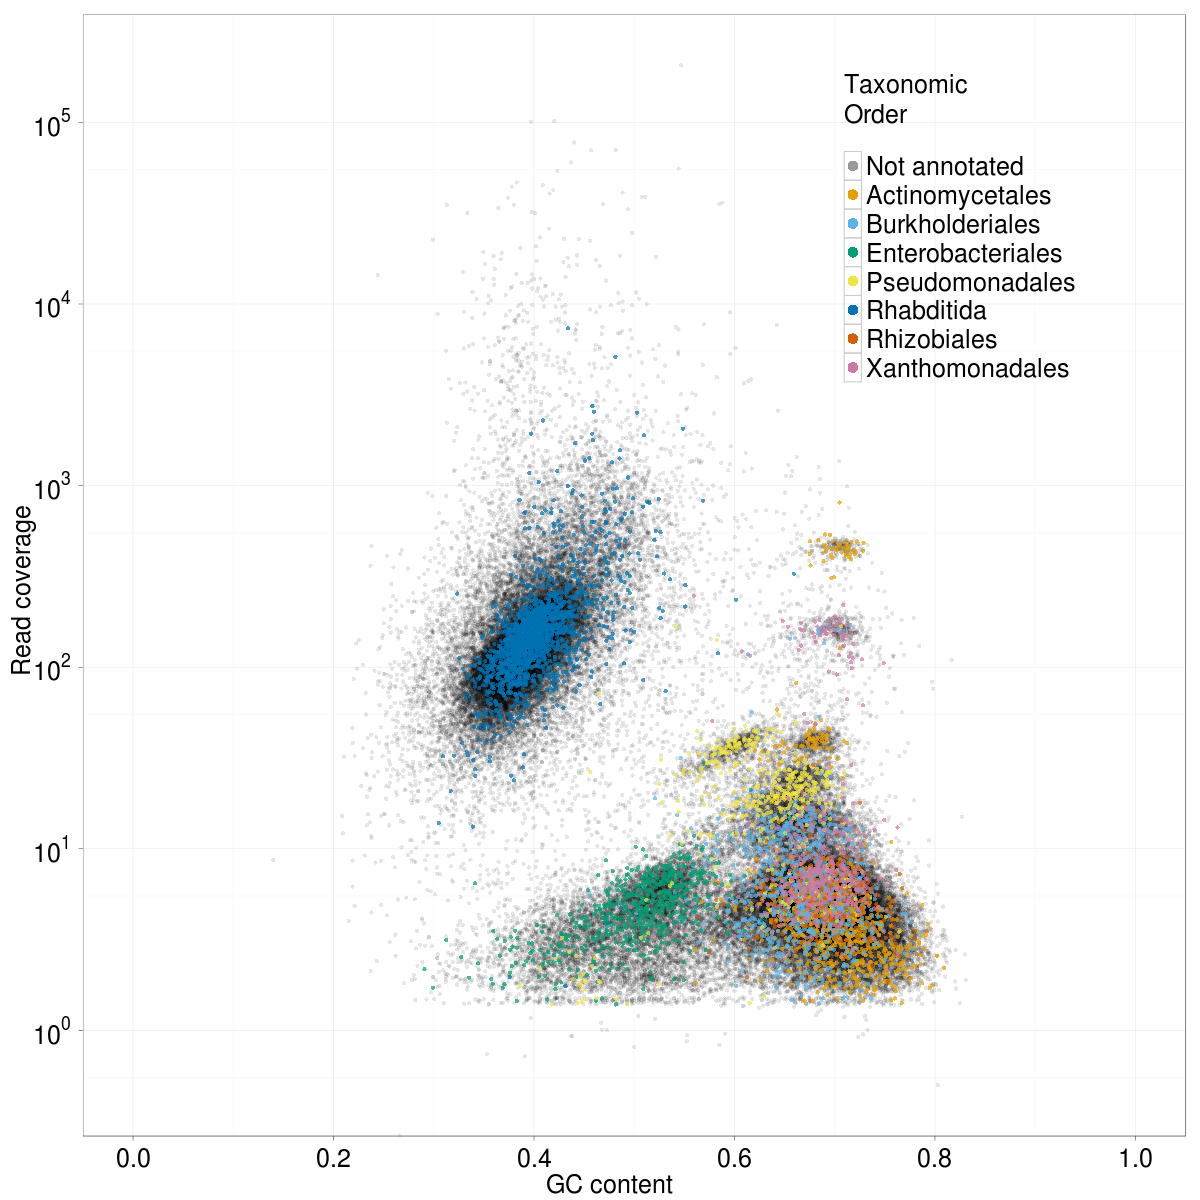
\includegraphics[width=1\textwidth]{images/blobology}
    \end{column}
  \end{columns}
\end{frame}

% k-mers
\begin{frame}
  \frametitle{$k$-mers}
     \begin{itemize}
       \item Nucleotides: \texttt{[ACGT]}
       \item Dinucleotides: \texttt{[AA|AC|AG|AT|CA|CC|$\ldots$]} (16 dimers)
       \item Trinucleotides: 32 trimers
       \item $k$-mers: $4^k$ $k$-mers
     \end{itemize}
     (see example in \texttt{data/shiny})
\end{frame}

% k-mer figures
\begin{frame}
  \frametitle{$k$-mers}
  Diagnostic differences in $k$-mer frequency, and variability.
  \begin{columns}[T]
    \begin{column}{5cm}
    \textit{E.coli}\\
     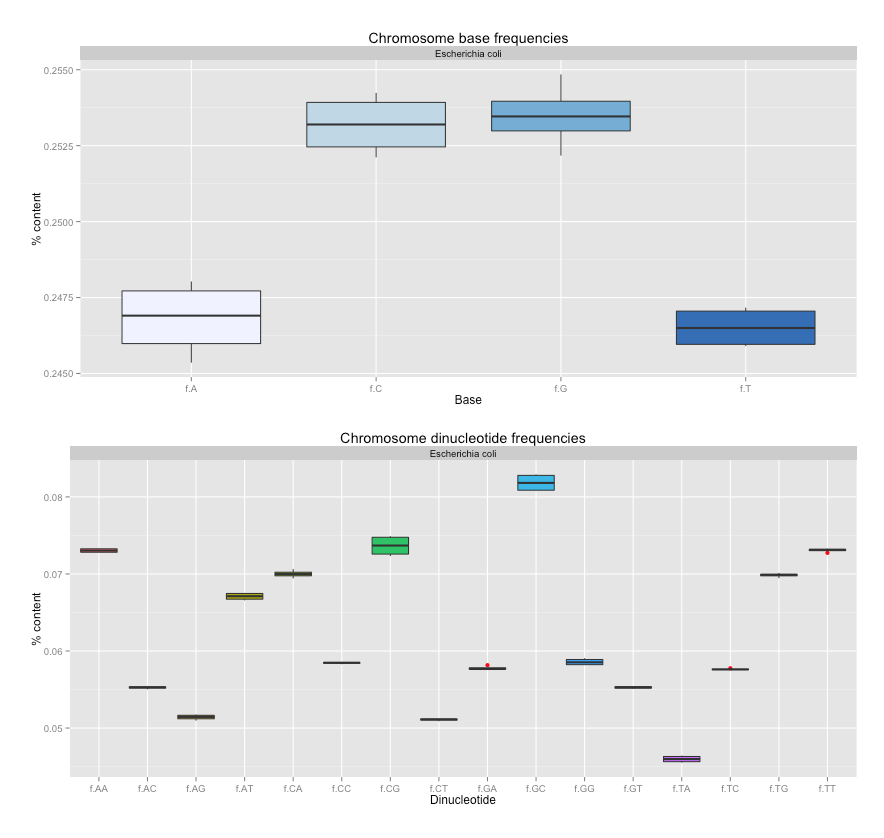
\includegraphics[width=1\textwidth]{images/kmer_ecoli}\\
    \end{column}
    \begin{column}{5cm}     
     \textit{Mycoplasma} spp.
     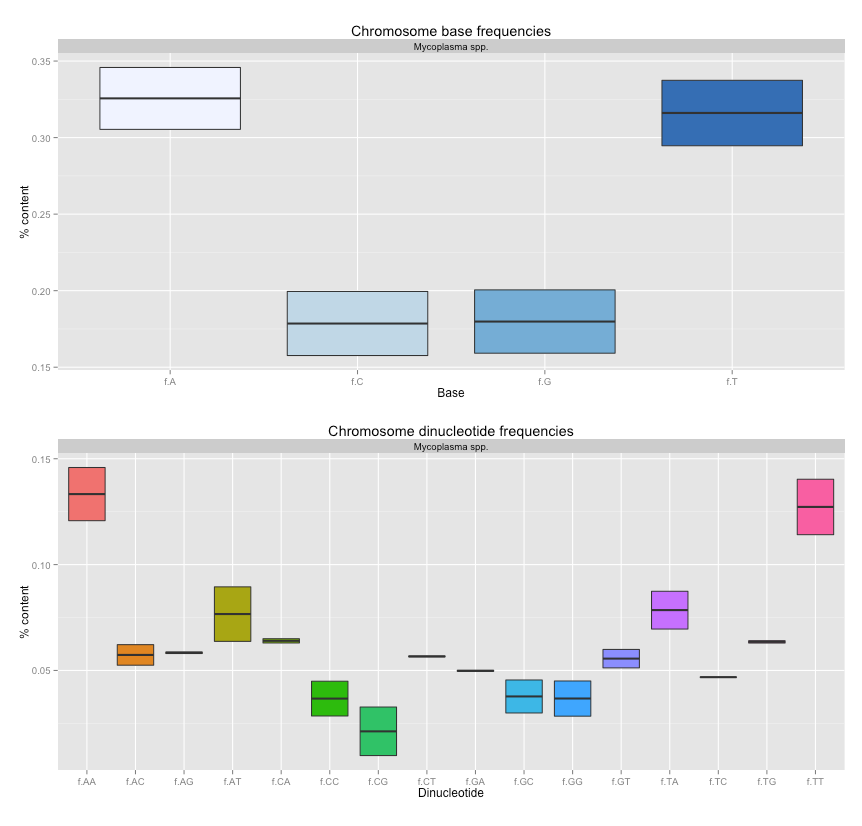
\includegraphics[width=1\textwidth]{images/kmer_mycoplasma}\\
   \end{column}
  \end{columns}
\end{frame}






%%%
% SECTION: Whole Genome Alignment
\section{Whole Genome Alignment}
%% whole_genome_alignment.tex
%% Author: Leighton Pritchard
%% Copyright: James Hutton Institute
%% A brief description of whole genome alignment and comparison


% SUBSECTION: Whole genome alignments
\subsection{An Introduction to Whole Genome Alignment}

% What do you align, and why?
\begin{frame}
  \frametitle{What to align, and why?}
  For useful analysis, the aligned genomes should:
  \begin{itemize}
    \item derive from a sufficiently recent common ancestor, so homologous regions can be identified
    \item derive from a sufficiently distant common ancestor, so that there are ``interesting'' differences to be identified
    \item \textbf{help to answer your biological question}: is your question organism or phenotype-specific? 
  \end{itemize}
  \begin{center}
    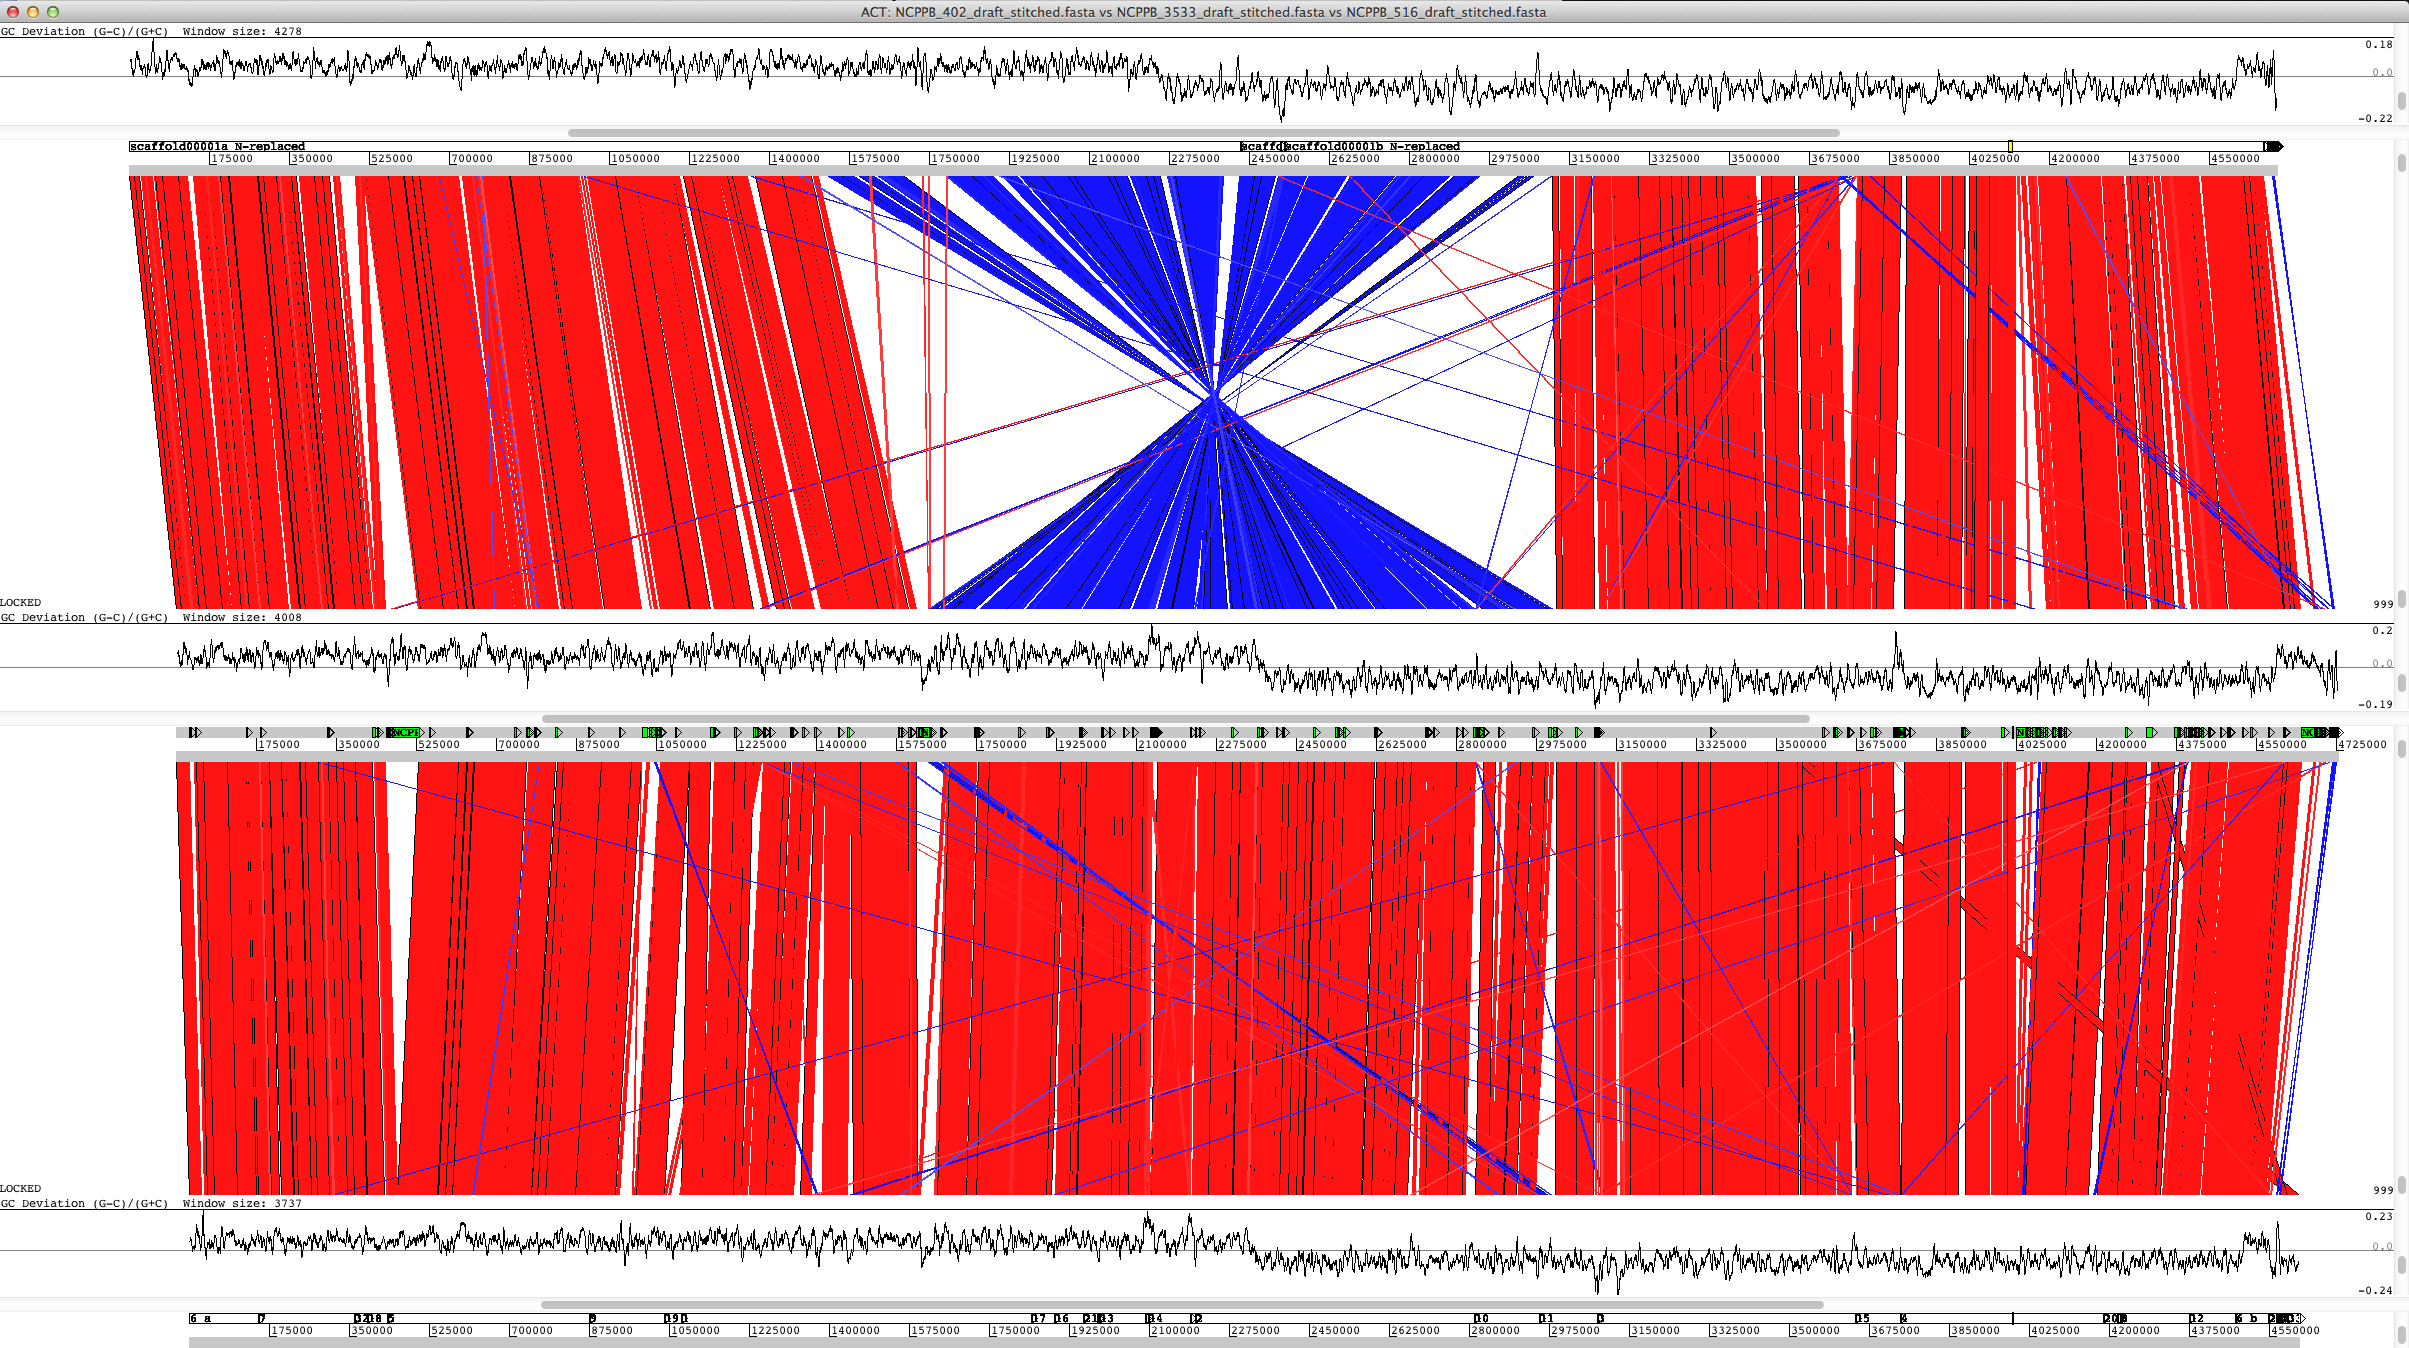
\includegraphics[width=0.6\textwidth]{images/act_comparison}
  \end{center}  
\end{frame}

% How do you align, and why?
\begin{frame}
  \frametitle{How to align, and why?}
  For useful analysis, the aligned genomes should:
  \begin{itemize}
    \item derive from a sufficiently recent common ancestor, so homologous regions can be identified
    \item derive from a sufficiently distant common ancestor, so that there are ``interesting'' differences to be identified
    \item \textbf{help to answer your biological question}: is your question organism or phenotype-specific? 
  \end{itemize}
  \begin{center}
    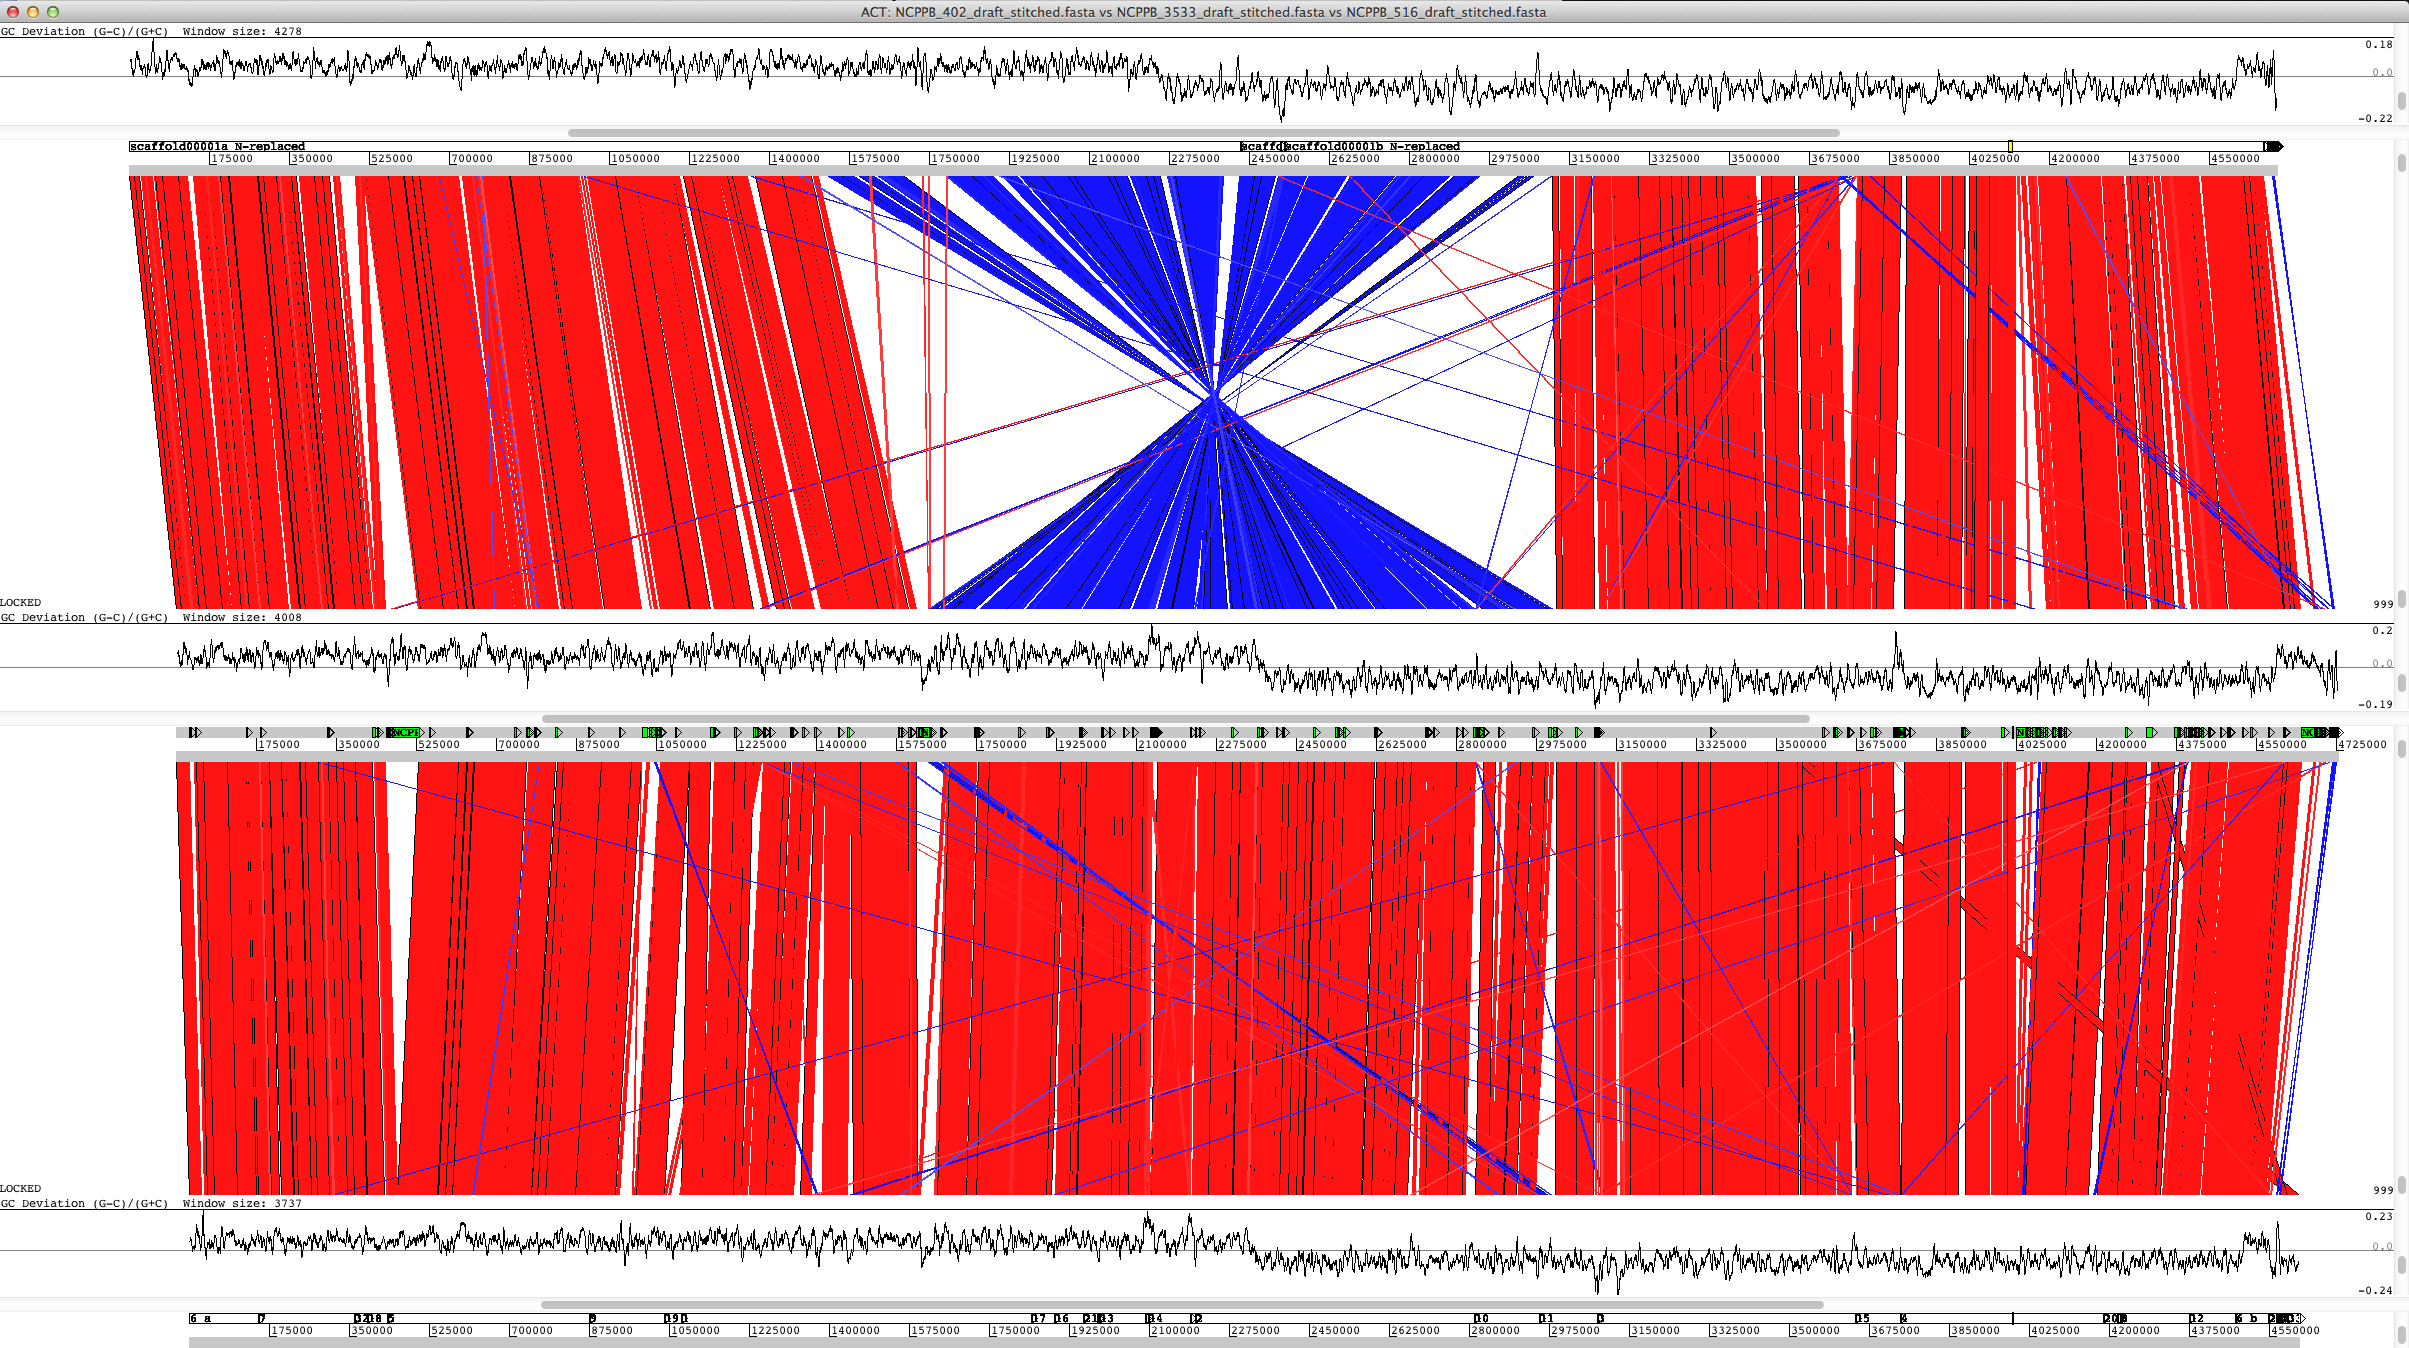
\includegraphics[width=0.6\textwidth]{images/act_comparison}
  \end{center}  
\end{frame}


% SUBSECTION: Average Nucleotide Identity
\subsection{Average Nucleotide Identity}

% DNA-DNA hybridisation
\begin{frame}
  \frametitle{DNA-DNA hybridisation\footnote{\tiny{\href{http://dx.doi.org/10.1016/S0168-6445(00)00040-1}{Morello-Mora and Amann (2001) \textit{FEMS Micro. Rev.} \textbf{25}:39-67 doi:10.1016/S0168-6445(00)00040-1}}}}
  \begin{columns}[T]
    \begin{column}{5cm}
      \begin{itemize}
        \item Denature DNA from two organisms.
        \item Allow to anneal. Reassociation $\approx$ similarity, measured as $\Delta T$  of denaturation curves.
        \item Proxy for sequence similarity.
        \item ``Gold Standard'' for prokaryotic taxonomy, since 1960s. ``70\% identity $\approx$ same species.''
      \end{itemize}
    \end{column}
    \begin{column}{5cm}
      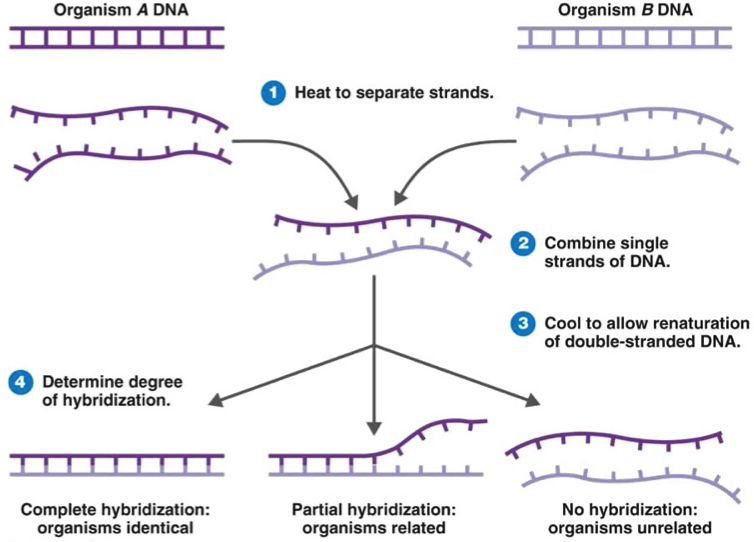
\includegraphics[width=1\textwidth]{images/ddh}
    \end{column}
  \end{columns}
\end{frame}

% ANIb
\begin{frame}
  \frametitle{Average Nucleotide Identity (ANIb)\footnote{\tiny{\href{http://dx.doi.org/10.1099/ijs.0.64483-0}{Goris \textit{et al}. (2007) \textit{Int. J. Syst. Biol.} \textbf{57}:81-91 doi:10.1099/ijs.0.64483-0}}}}
  \begin{columns}[T]
    \begin{column}{5cm}
      1. Break genomes into 1020t fragments\\
      2. \textbf{ANIb}: Mean \% identity of all BLASTN matches with $>30\%$ identity and $>70\%$ fragment coverage.\\[0.5cm]
      \begin{itemize}
        \item DDH:ANIb linear
        \item DDH:\%ID linear
        \item 70\%ID $\approx$ 95\%ANIb
      \end{itemize}
    \end{column}
    \begin{column}{5cm}
      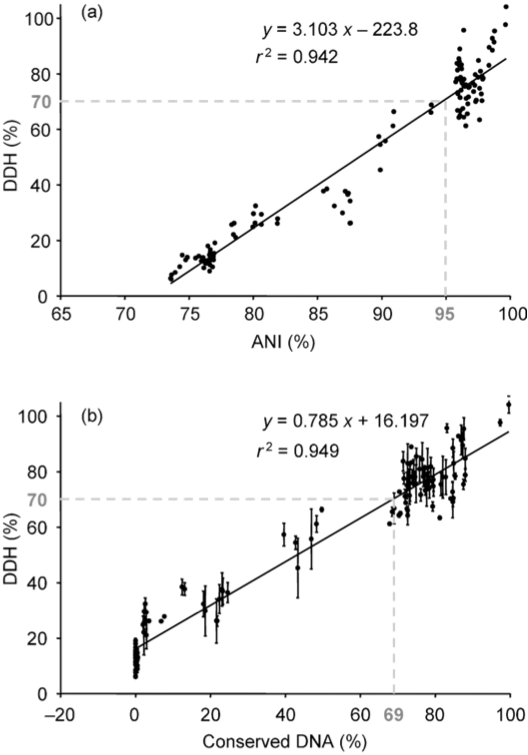
\includegraphics[width=1\textwidth]{images/ddh_ani_pid}
    \end{column}
  \end{columns}
\end{frame}

% ANIm
\begin{frame}
  \frametitle{Average Nucleotide Identity (ANIm)\footnote{\tiny{\href{http://dx.doi.org/10.1073/pnas.0906412106}{Richter and Rossello-Mora (2009) \textit{Proc. Natl. Acad. Sci. USA} \textbf{106}:19126-19131 doi:10.1073/pnas.0906412106}}}}
  \begin{columns}[T]
    \begin{column}{3cm}
      1. Align genomes with MUMmer\\
      2. \textbf{ANIm}: Mean \% identity of all matches\\[0.25cm]
      \begin{itemize}
        \item DDH:ANIm linear
        \item 70\%ID $\approx$ 95\%ANIb
      \end{itemize}
    \end{column}
    \begin{column}{7cm}
      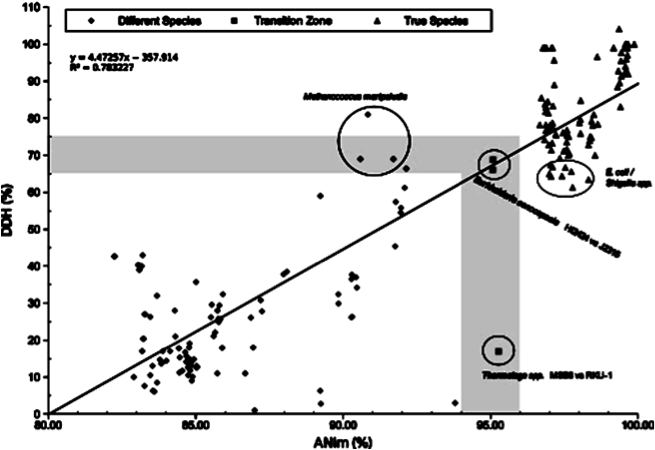
\includegraphics[width=1\textwidth]{images/ddh_anim}
    \end{column}
  \end{columns}
  \textbf{TETRA}: tetranucleotide frequency-based classifier introduced in same paper.
\end{frame}

% ANIb/ANIm/TETRA comparison
\begin{frame}
  \frametitle{ANI/TETRA comparison}
  All three methods applied to \textit{Anaplasma} spp.\\[0.25cm]
  \begin{columns}[T]
    \begin{column}{4cm}
    ANIb:\\
      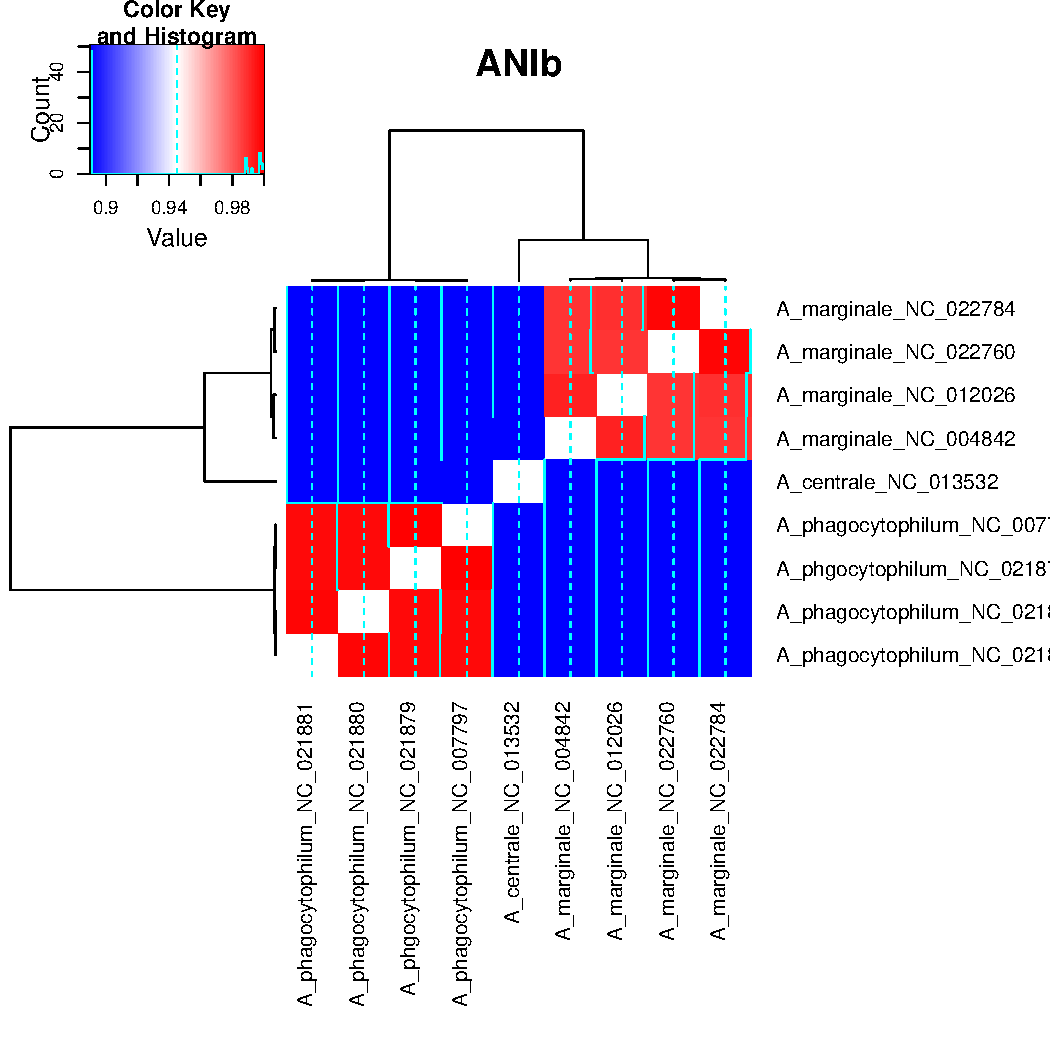
\includegraphics[width=1\textwidth]{images/ANIb}
    \end{column}
    \begin{column}{4cm}
    ANIm:\\
      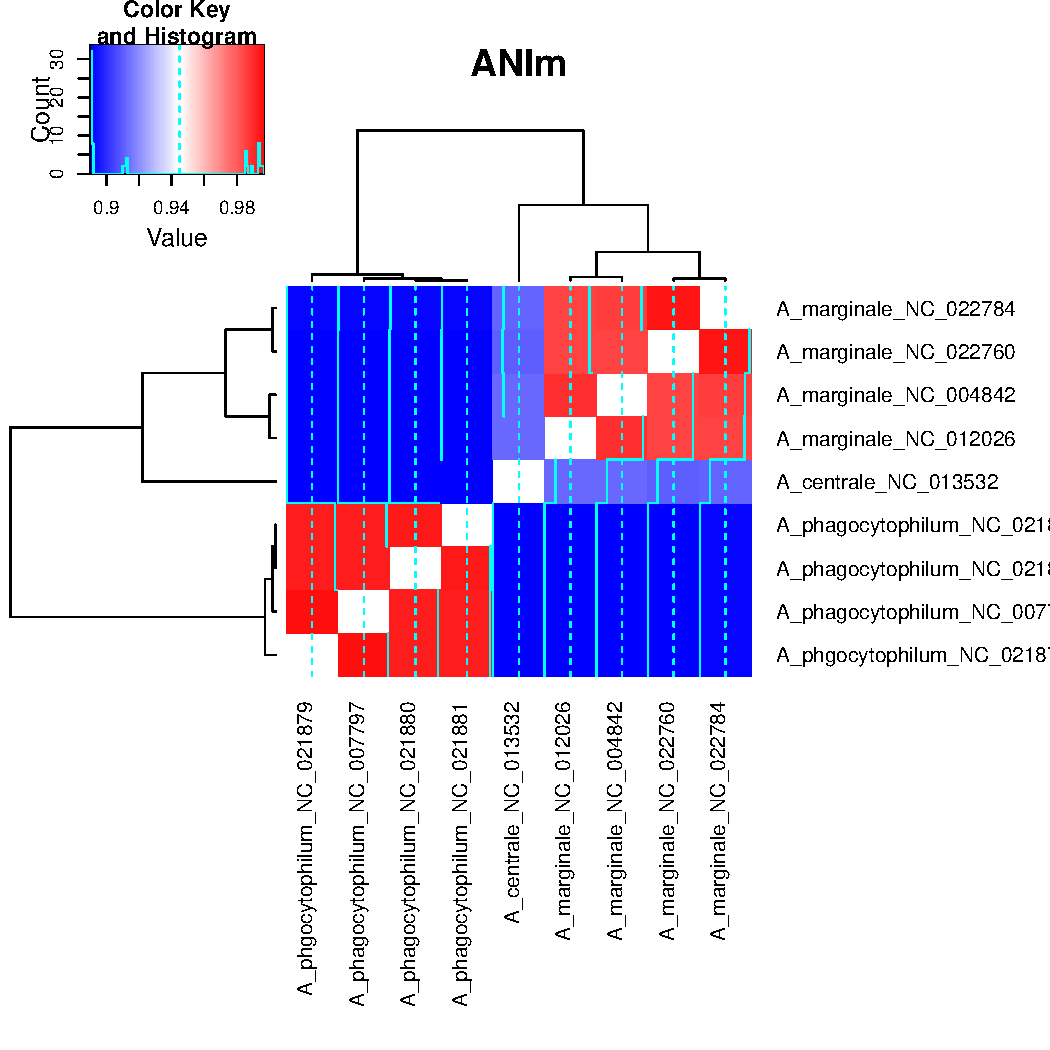
\includegraphics[width=1\textwidth]{images/ANIm}
    \end{column}
    \begin{column}{4cm}   
    TETRA:\\
      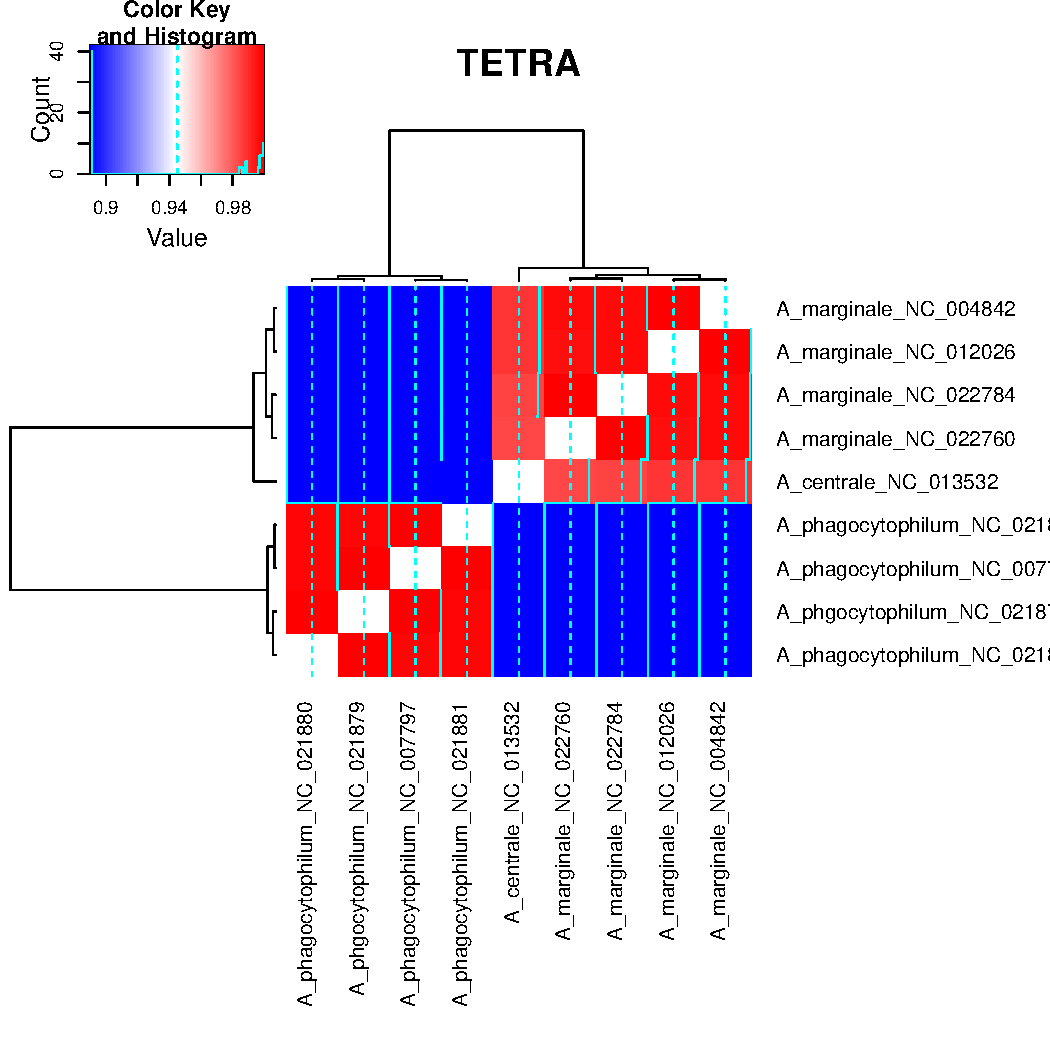
\includegraphics[width=1\textwidth]{images/TETRA}
    \end{column}
  \end{columns}       
  ANIb discards information, relative to ANIm\\
  ANIb/ANIm reflect evolutionary history; TETRA reflects bulk composition
\end{frame}

% ANIm in practice
\begin{frame}
  \frametitle{ANI in practice}
  Two practical applications\\[0.25cm]
  \begin{columns}[T]
    \begin{column}{6cm}
    29 \textit{Dickeya} isolates:\\
    More complex species structure\\
      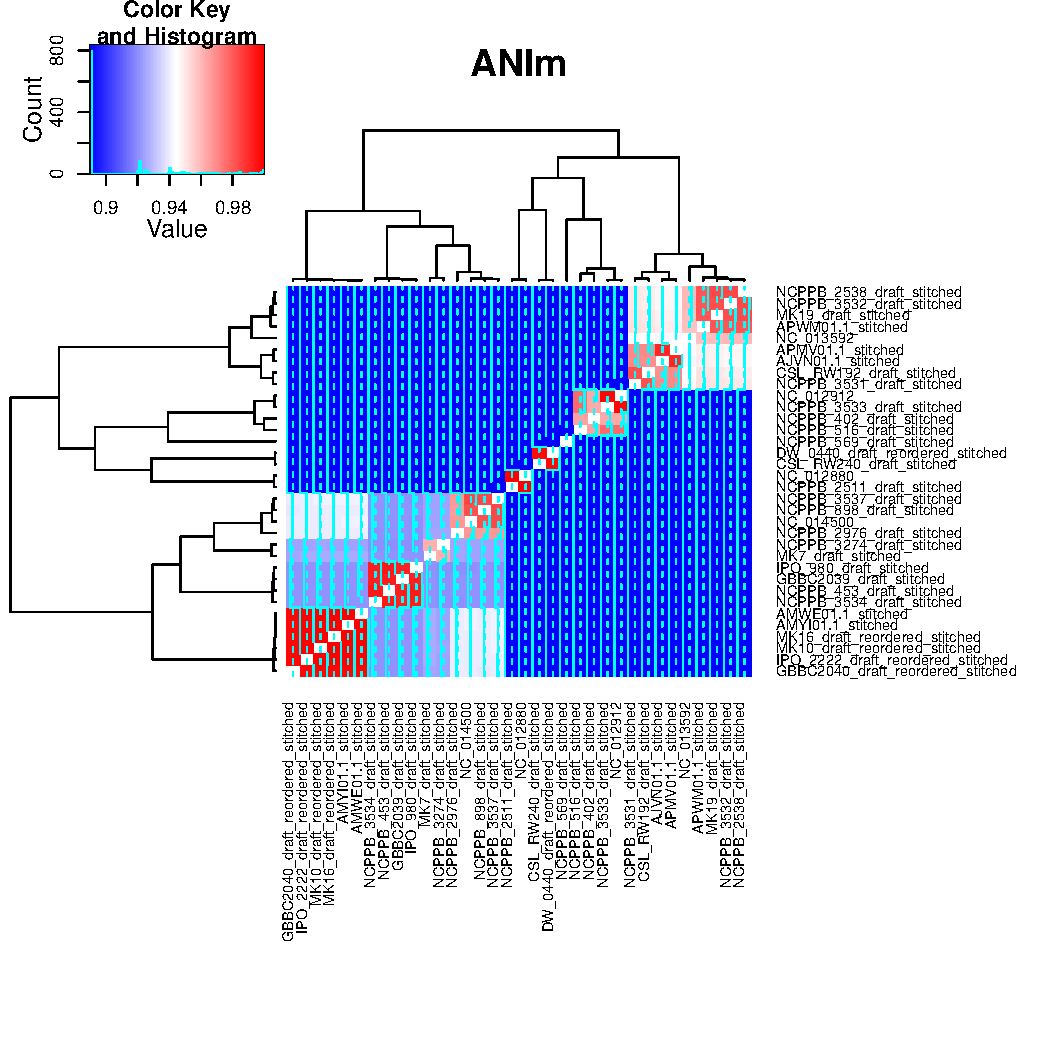
\includegraphics[width=1\textwidth]{images/ANIm_Dickeya}
    \end{column}
    \begin{column}{6cm}
    180 \textit{E.coli} isolates:\\
    More complex subtyping
      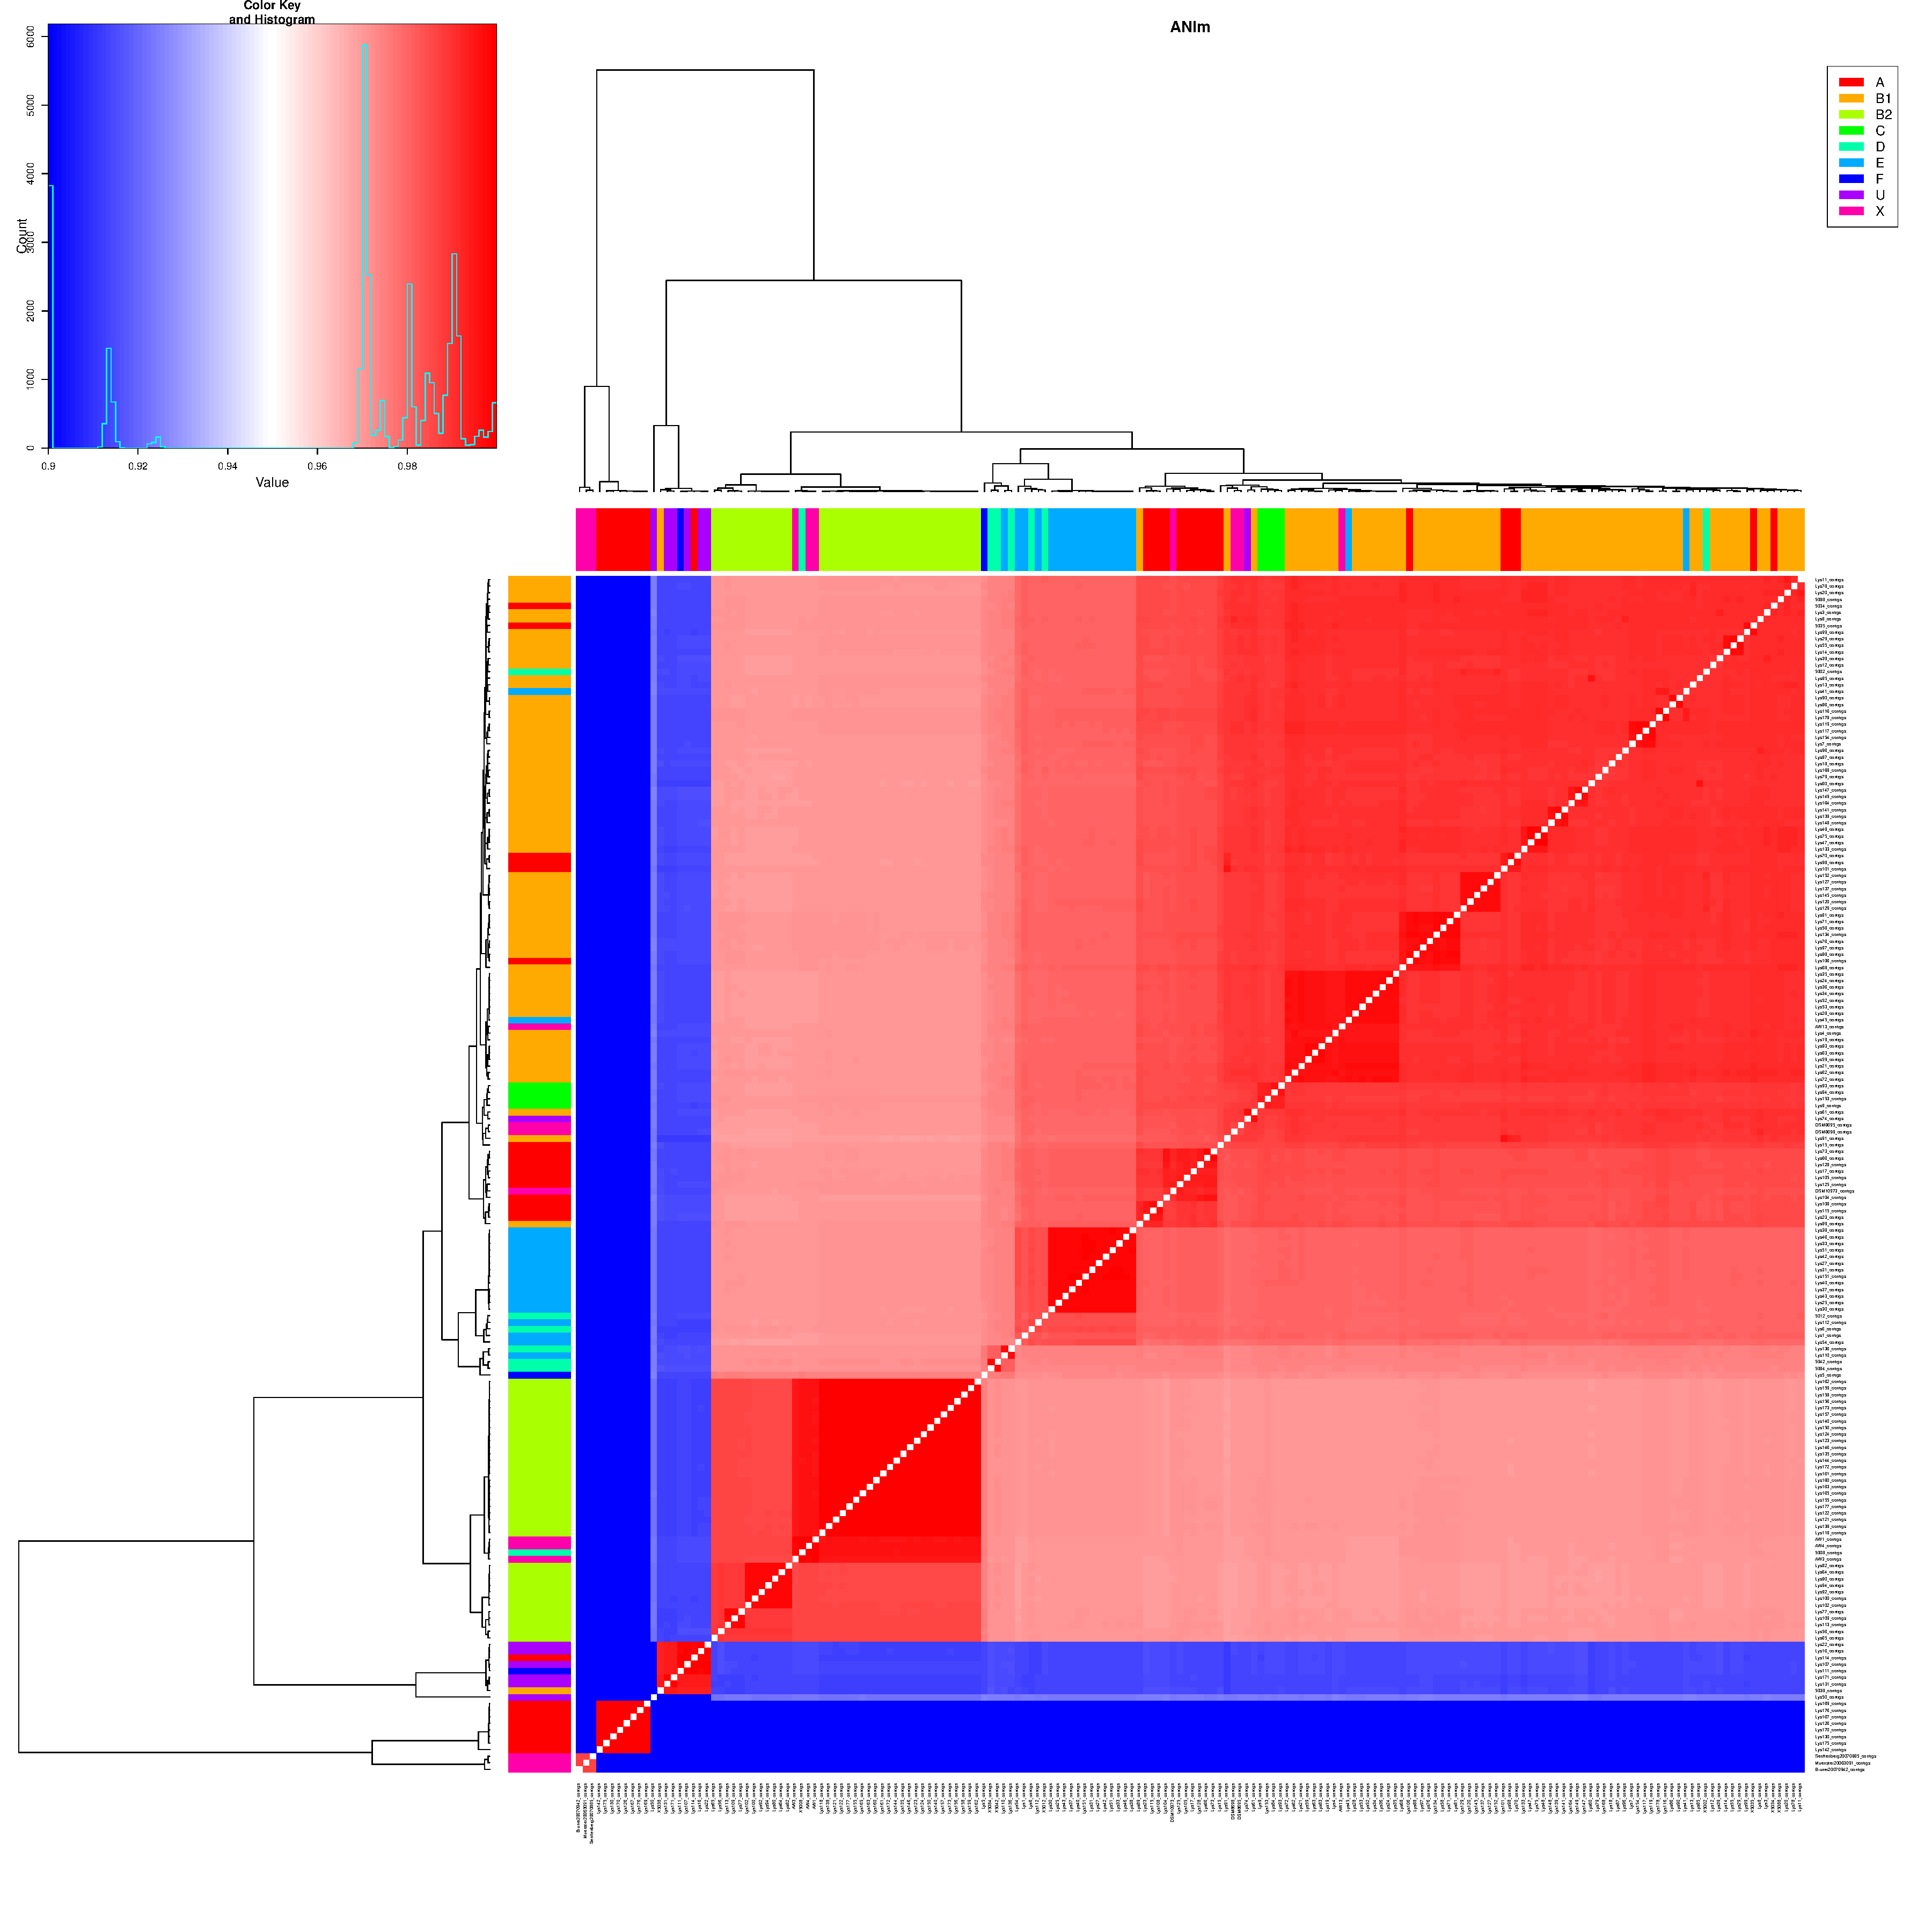
\includegraphics[width=1\textwidth]{images/ANIm_Ecoli}
    \end{column}
  \end{columns}       
\end{frame}

%%%
% SECTION: Collinearity and Synteny
%\section{Collinearity and Synteny}
%\input{sections/collinearity_and_synteny}


%%%
% ACKNOWLEDGEMENTS
%\section{Acknowledgements}
%\input{sections/acknowledgements}


%%%
% LICENCE FOR REUSE
%% licence.tex
%% Author: Leighton Pritchard
%% Copyright: James Hutton Institute
%% These slides describe the licence for reuse of these slides and
%% materials

%
\begin{frame}
  \frametitle{Licence: CC-BY-SA}
  By: Leighton Pritchard \\[0.5cm]
  This presentation is licensed under the Creative Commons Attribution ShareAlike license \\
  \href{https://creativecommons.org/licenses/by-sa/4.0/}{https://creativecommons.org/licenses/by-sa/4.0/}
\end{frame}

% etc
\end{document}